% ============================================================
%  Mid-semester Project Review -- Beamer slides
%  Composing Context Compression for Long-Horizon LLM Agents
%  Compile with: pdflatex midreview_slides.tex  (run twice)
% ============================================================
\documentclass[aspectratio=169,10pt]{beamer}

\usetheme{Madrid}
\usecolortheme{default}
\setbeamertemplate{navigation symbols}{}
\setbeamertemplate{frametitle continuation}{}
\setbeamertemplate{caption}[numbered]
\setbeamerfont{block title}{size=\normalsize}
\setbeamertemplate{itemize items}[circle]

\usepackage[T1]{fontenc}
\usepackage{lmodern}
\usepackage{amsmath,amssymb,mathtools}
\usepackage{booktabs}
\usepackage{graphicx}
\usepackage{tikz}
\usetikzlibrary{arrows.meta,positioning,calc,fit,shapes.geometric}
\usepackage{pgfplots}
\pgfplotsset{compat=1.16}

% tighter lists
\setlength{\leftmargini}{1.4em}
\setlength{\leftmarginii}{1.2em}

% shorthand colours used across the diagrams
\definecolor{envblue}{RGB}{31,80,140}
\definecolor{cmpgreen}{RGB}{28,110,60}
\definecolor{ctlorange}{RGB}{190,105,10}
\definecolor{metviolet}{RGB}{110,45,140}

\title[Composing Context Compression]{Composing Context Compression\\for Long-Horizon LLM Agents}
\subtitle{Controlled Composition and Critical-Fact Retention on top of ACON}

\author[Ayush Rahate \& Rohit Chauhan]{
  \begin{tabular}{r@{\hspace{0.8em}}l}
    \textbf{123CS0006} & Ayush Rahate\\
    \textbf{123CS0054} & Rohit Chauhan
  \end{tabular}
}

\institute[IIITDM Kurnool]{
  Department of Computer Science and Engineering\\
  Indian Institute of Information Technology\\
  Design and Manufacturing, Kurnool
}

\date[Mid-Sem Review]{Mid-Semester Project Review \\ September 2026}

% ------------------------------------------------------------
\begin{document}

% ============================== 1. TITLE
{
\setbeamertemplate{footline}{}
\begin{frame}[plain]
  \vspace{-0.3cm}
  \begin{center}
    \includegraphics[height=1.25cm]{"png college logo".png}
  \end{center}
  \vspace{-0.55cm}
  {\setbeamerfont{title}{size=\large,series=\bfseries}%
   \setbeamerfont{subtitle}{size=\scriptsize}%
   \setbeamerfont{author}{size=\scriptsize}%
   \setbeamerfont{institute}{size=\tiny}%
   \setbeamerfont{date}{size=\tiny}%
   \titlepage}
  \vspace{-0.85cm}
  \begin{center}
    \scriptsize\textbf{Project Supervisor:} Dr.~N.~Srinivas Naik
  \end{center}
\end{frame}
}

% ============================== 2. OUTLINE
\begin{frame}{Outline}
  \tableofcontents
\end{frame}

% ============================== 3. MOTIVATION
\section{Motivation}

\begin{frame}{The Problem: Context Grows Without Bound}
\begin{columns}[T]
\begin{column}{0.52\textwidth}
\centering
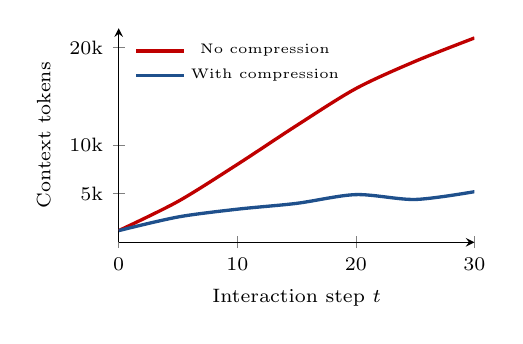
\begin{tikzpicture}[font=\scriptsize]
\begin{axis}[
  width=6.1cm, height=4.3cm,
  xlabel={Interaction step $t$},
  ylabel={Context tokens},
  xmin=0, xmax=30, ymin=0, ymax=22000,
  ytick={5000,10000,20000},
  yticklabels={5k,10k,20k},
  scaled y ticks=false,
  xtick={0,10,20,30},
  axis lines=left,
  legend style={at={(0.02,0.98)},anchor=north west,draw=none,fill=none,font=\tiny},
]
\addplot[red!75!black, very thick, smooth] coordinates {
  (0,1200)(5,4200)(10,8000)(15,12000)(20,15800)(25,18600)(30,21000)};
\addlegendentry{No compression}
\addplot[envblue, very thick, smooth] coordinates {
  (0,1200)(5,2600)(10,3400)(15,4000)(20,4900)(25,4400)(30,5200)};
\addlegendentry{With compression}
\end{axis}
\end{tikzpicture}
\end{column}
\begin{column}{0.46\textwidth}
\begin{alertblock}{Two bottlenecks}
\begin{itemize}\footnotesize
  \item \textbf{Memory} --- the KV cache scales with sequence length
  \item \textbf{Distraction} --- long, partly stale context degrades decisions
\end{itemize}
\end{alertblock}
\begin{block}{The tension}
\footnotesize
Compression must be \emph{aggressive} (to save tokens) and \emph{precise}
(one lost file path or API token derails an entire trajectory).
\end{block}
\end{column}
\end{columns}
\end{frame}

% ============================== 4. BACKGROUND
\section{Background and Related Work}

\begin{frame}{The Two Methods We Build On}
\begin{columns}[T]
\begin{column}{0.49\textwidth}
\begin{block}{ACON --- prompt-level, generative}
\footnotesize
\begin{itemize}
  \item An LLM \emph{rewrites} the history when $|h_t| > T_{\mathrm{hist}}$
        and shortens observations when $|o_t| > T_{\mathrm{obs}}$
  \item The compression guideline is optimised \emph{in natural language}:
        contrast runs that succeed uncompressed but fail compressed
  \item Agent weights stay frozen; compressor is distilled into a small model
  \item AppWorld: $56.5\%$ vs.\ $56.0\%$ accuracy, peak tokens $\downarrow$ 26--54\%
\end{itemize}
\end{block}
\end{column}
\begin{column}{0.49\textwidth}
\begin{block}{SAC --- KV-level, soft}
\footnotesize
\begin{itemize}
  \item Selects \emph{anchor tokens}, marks them with a learned embedding
  \item Bidirectional attention lets anchor KV pairs absorb the whole context
  \item No autoencoding pretraining required
  \item MRQA, Llama-3.2-1B at $15\times$: $54.95$ in-domain F1 (vs.\ EPL $51.52$)
\end{itemize}
\end{block}
\end{column}
\end{columns}
\vspace{0.25cm}
\begin{center}
\footnotesize
Our project \textbf{reproduces both on our own hardware}, then asks how
compression stages should be \emph{composed} and \emph{evaluated}.
\end{center}
\end{frame}

% ============================== 5. LITERATURE TABLE
\begin{frame}{Where the Field Stands}
\centering
\scriptsize
\renewcommand{\arraystretch}{1.25}
\setlength{\tabcolsep}{3.5pt}
\resizebox{\textwidth}{!}{%
\begin{tabular}{lcccccc}
\toprule
\textbf{Property} & \textbf{ACON} & \textbf{SAC} & \textbf{SWE-Pruner} &
\textbf{LLMLingua} & \textbf{MEM1/MemAgent} & \textbf{Proposed}\\
\midrule
Output form              & Text & KV cache & Text lines & Text tokens & Text memory & Text\\
Agent weights frozen     & Yes  & Yes & Yes & Yes & \textcolor{red!70!black}{No} & Yes\\
History compression      & Yes  & No  & No  & Yes & Merged & Yes\\
Observation compression  & Yes  & No  & Yes & Yes & Merged & Yes\\
Composition studied      & Partly & No & No & No & No & \textcolor{cmpgreen}{\textbf{Yes}}\\
Intrinsic quality metric & No   & No  & No  & No  & No & \textcolor{cmpgreen}{\textbf{Yes (CFR)}}\\
\bottomrule
\end{tabular}}



\vspace{0.4cm}
\begin{columns}
\begin{column}{0.88\textwidth}
\footnotesize
\begin{itemize}
  \item ``Partly'': ACON reports a combined setting in an appendix ablation only.
  \item ``Merged'': a single learned memory holds both history and observations.
  \item Every existing method compresses \emph{one} kind of context ---
        how the stages \textbf{interact} is unstudied.
\end{itemize}
\end{column}
\end{columns}
\end{frame}

% ============================== 6. SETUP
\section{Reproduction}

\begin{frame}{Experimental Setup}
\begin{columns}[T]
\begin{column}{0.48\textwidth}
\begin{block}{Hardware \& serving}
\footnotesize
\begin{itemize}
  \item One NVIDIA RTX 2000 Ada (16\,GB)
  \item Models served locally through Ollama
  \item Agent: \texttt{qwen2.5:14b}
  \item Compressor: \texttt{qwen2.5:7b}
\end{itemize}
\end{block}
\begin{block}{Benchmarks}
\footnotesize
\begin{itemize}
  \item \textbf{ACON:} AppWorld \texttt{train\_history\_tiny} (38 tasks),
        seed 42, temperature 0
  \item \textbf{SAC:} authors' Llama-3.2-1B checkpoints on MRQA
\end{itemize}
\end{block}
\end{column}
\begin{column}{0.48\textwidth}
\begin{alertblock}{Deviations from the papers --- and why}
\footnotesize
\begin{itemize}
  \item Thresholds $T_{\mathrm{hist}}{=}512$, $T_{\mathrm{obs}}{=}256$
        instead of $4096/1024$ --- the paper values almost never fire
        on this split
  \item Ollama served both models with a \textbf{4096-token} context, so long
        baseline prompts were truncated
  \item One seed per setting so far
\end{itemize}
\end{alertblock}
\vspace{0.1cm}
\footnotesize
These caveats are carried explicitly into every claim that follows.
\end{column}
\end{columns}
\end{frame}

% ============================== 7. ACON RESULTS
\begin{frame}{Result 1: ACON Reproduction on AppWorld}
\centering
\scriptsize
\renewcommand{\arraystretch}{1.2}
\setlength{\tabcolsep}{4.5pt}
\resizebox{\textwidth}{!}{%
\begin{tabular}{lcccccc}
\toprule
\textbf{Run} & \textbf{Tasks} & \textbf{Max iter.} & \textbf{Solved} &
\textbf{Avg iter.} & \textbf{Agent input tok.} & \textbf{Wall clock (s)}\\
\midrule
Baseline, no compression                          & 8  & 12 & 1 & 11.00 & 269,935 & 953.9\\
History compression ($T_{\mathrm{hist}}{=}512$)   & 8  & 12 & \textbf{2} & 10.75 & 232,749 & 882.8\\
Observation compression ($T_{\mathrm{obs}}{=}256$)& 8  & 12 & 1 & 11.00 & 261,422 & 873.6\\
\midrule
Baseline, full split                              & 38 & 30 & 12 (31.6\%) & 23.7 & 2,972,376 & 7312\\
\midrule
Baseline, matched subset                          & 18 & 30 & 7 & 22.22 & 1,283,906 & ---\\
History compression, matched subset               & 18 & 30 & \textbf{9} & 19.50 & \textbf{969,389} & ---\\
\bottomrule
\end{tabular}}


\vspace{0.35cm}
\begin{columns}
\begin{column}{0.92\textwidth}
\footnotesize
\begin{itemize}
  \item On the 18 matched tasks: \textbf{9 solved vs.\ 7}, with
        \textbf{24.5\% fewer agent input tokens}.
  \item The change is \emph{not uniform} --- it solved 5 tasks the baseline
        failed, and failed 3 the baseline solved.
  \item At this scale the latency overhead ACON reports did \textbf{not} appear;
        all compressed runs finished sooner.
\end{itemize}
\end{column}
\end{columns}
\end{frame}

% ============================== 8. SAC RESULTS
\begin{frame}{Result 2: SAC Reproduction and the SAC\,$\times$\,ACON Pilot}
\begin{block}{SAC reproduces to within 0.2 F1}
\footnotesize
$15\times$: \textbf{54.98} ID / \textbf{39.25} OOD (published 54.95 / 39.26)
\qquad
$5\times$: \textbf{63.70} / \textbf{47.71} (published 63.63 / 47.72)
\end{block}
\vspace{-0.1cm}
\centering
\scriptsize
\renewcommand{\arraystretch}{1.2}
\setlength{\tabcolsep}{4.5pt}
\resizebox{\textwidth}{!}{%
\begin{tabular}{lcccc}
\toprule
\textbf{Run} & \textbf{ID F1} & \textbf{OOD F1} &
\textbf{$\Delta$ID vs.\ R0 (95\% CI)} & \textbf{$\Delta$OOD vs.\ R0 (95\% CI)}\\
\midrule
R0: SAC fine-tuning (matched control)  & 51.37 & 38.62 & control & control\\
R1: $+$ uniform KL (ablation)          & 51.06 & 38.17 & $-0.32\ [-1.02,+0.44]$ & $-0.45\ [-2.11,+1.44]$\\
R2: $+$ FGD (gated KL, $\lambda{=}1$)  & 51.15 & 38.47 & $-0.23\ [-0.95,+0.47]$ & $-0.14\ [-2.04,+1.77]$\\
R3: $+$ TGA $+$ FGD                    & \textbf{60.03} & \textbf{44.71} &
   $\mathbf{+8.66}\ [+7.66,+9.60]$ & $\mathbf{+6.10}\ [+3.62,+8.96]$\\
\midrule
\emph{Published SAC $15\times$ (20{,}000 steps)} & \emph{54.95} & \emph{39.26} & &\\
\bottomrule
\end{tabular}}



\vspace{0.3cm}
\begin{columns}
\begin{column}{0.92\textwidth}
\footnotesize
\begin{itemize}
  \item \textbf{FGD is a null result.} Its intervals contain zero. A diagnostic
        explains why: the zero-shot full-context teacher had \emph{higher}
        gold-answer NLL than the compressed student on \textbf{90.5\%} of
        2,000 training examples --- there is little to distil.
  \item \textbf{TGA\,$+$\,FGD wins}, beating the published 20,000-step
        checkpoint after a quarter of the budget --- but the question is seen
        during compression, so the memory is \emph{not reusable} across
        questions. This is a separate query-aware setting, not a drop-in
        improvement.
\end{itemize}
\end{column}
\end{columns}
\end{frame}

% ============================== 9. GAP A
\section{Research Gaps}

\begin{frame}{Gap (a): Token Savings Do Not Become Time Savings}
\begin{columns}[T]
\begin{column}{0.47\textwidth}
\centering
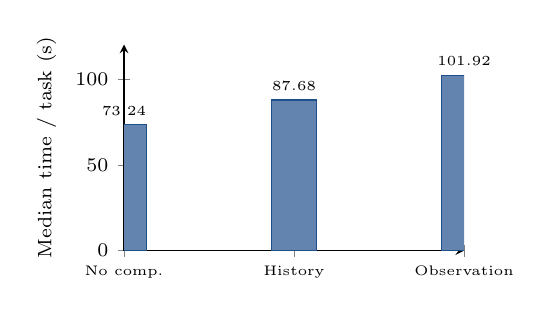
\begin{tikzpicture}[font=\scriptsize]
\begin{axis}[
  width=5.9cm, height=4.2cm,
  ybar, bar width=16pt,
  ylabel={Median time / task (s)},
  symbolic x coords={No comp., History, Observation},
  xtick=data,
  ymin=0, ymax=120,
  nodes near coords, nodes near coords style={font=\tiny},
  x tick label style={font=\tiny},
  axis lines=left,
]
\addplot[fill=envblue!70, draw=envblue] coordinates {
  (No comp.,73.24) (History,87.68) (Observation,101.92)};
\end{axis}
\end{tikzpicture}

{\tiny ACON's own measurement: Qwen3-14B agent \& compressor, one A100.}
\end{column}
\begin{column}{0.51\textwidth}
\begin{alertblock}{Why compression can cost time}
\footnotesize
\begin{itemize}
  \item The compressor generates \textbf{autoregressively} --- it is itself an
        LLM call
  \item Rewriting the history \textbf{invalidates the agent's KV cache}, so the
        compressed prefix must be re-encoded from scratch
\end{itemize}
\end{alertblock}
\begin{block}{Consequence}
\footnotesize
A token-count objective $C(\pi)$ does not capture this overhead at all.
Latency must be modelled as a \emph{separate} term.
\end{block}
\end{column}
\end{columns}
\end{frame}

% ============================== 10. GAP B
\begin{frame}{Gap (b): The Combined Setting Is Schedule-Confounded}
\begin{block}{The trigger set depends on the pipeline itself}
\footnotesize
\[
\mathcal{K}(\pi)=\big\{\,t \;:\; |h'_{t-1}\oplus(o'_t,a_t)|>T_{\mathrm{hist}}\,\big\}
\]
Since $|o'_t|\le|o_t|$, compressing observations first makes $|h_t|$ grow more
slowly. History compression then fires at \textbf{different steps}, and on
\textbf{already-pruned text}: in general
$\mathcal{K}(\pi_{ho})\neq\mathcal{K}(\pi_{h})$.
\end{block}

\begin{columns}[T]
\begin{column}{0.46\textwidth}
\begin{block}{The interaction term}
\footnotesize
\[
I=\Delta(\pi_{ho})-\Delta(\pi_h)-\Delta(\pi_o)
\]
On AppWorld: $\Delta(\pi_h)={+}0.5$, $\Delta(\pi_o)={-}2.4$ and
$\Delta(\pi_{ho})={-}11.4$ points, so
\[
I=\mathbf{-9.5}\ \text{points.}
\]
\end{block}
\end{column}
\begin{column}{0.50\textwidth}
\begin{alertblock}{Why this number cannot be interpreted}
\footnotesize
$I$ mixes \emph{two} effects that change simultaneously:
\begin{enumerate}
  \item genuinely composing $f_o$ with $f_h$
  \item the \textbf{shifted trigger schedule}
\end{enumerate}
The two cannot be separated, so $-9.5$ is \emph{not} evidence that composition
itself is harmful.
\end{alertblock}
\end{column}
\end{columns}
\end{frame}

% ============================== 11. GAP C
\begin{frame}{Gap (c): Compression Quality Is Only Measured Indirectly}
\begin{center}
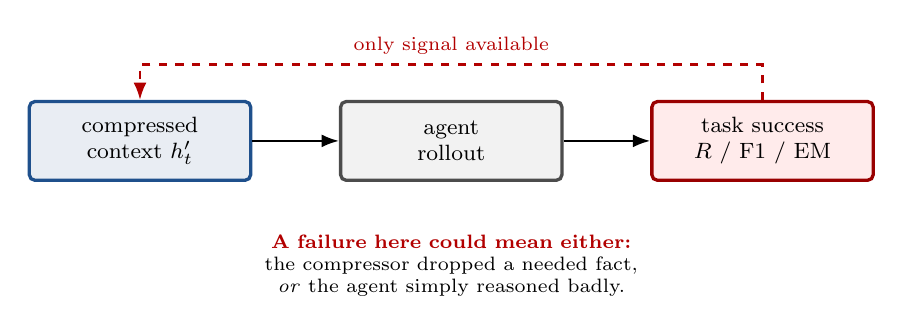
\begin{tikzpicture}[
  font=\footnotesize,
  bx/.style={draw, rounded corners=2pt, very thick, align=center,
             text width=2.6cm, minimum height=1.0cm, inner sep=3pt},
  arr/.style={-{Latex[length=2.2mm]}, line width=0.8pt}
]
\node[bx, fill=envblue!10, draw=envblue] (c)  {compressed\\context $h'_t$};
\node[bx, fill=gray!10, draw=gray!60!black, right=1.1cm of c] (a) {agent\\rollout};
\node[bx, fill=red!8, draw=red!60!black, right=1.1cm of a] (r) {task success\\$R$ / F1 / EM};
\draw[arr] (c)--(a);
\draw[arr] (a)--(r);
\node[below=0.55cm of a, font=\scriptsize, text width=6.5cm, align=center]
  {\textcolor{red!70!black}{\textbf{A failure here could mean either:}}\\
   the compressor dropped a needed fact, \emph{or} the agent simply reasoned badly.};
\draw[arr, dashed, red!70!black] (r.north) -- ++(0,0.45) -| node[pos=0.25,above,font=\scriptsize]
  {only signal available} (c.north);
\end{tikzpicture}
\end{center}
\vspace{0.1cm}
\begin{columns}
\begin{column}{0.9\textwidth}
\footnotesize
\begin{itemize}
  \item ACON and SAC judge a compressor \textbf{solely} by downstream success.
  \item Neither measures whether the \emph{specific facts the agent will need}
        survive compression.
  \item So a failure \textbf{cannot be attributed} to information loss rather
        than to the agent --- the compressor is never diagnosed directly.
\end{itemize}
\end{column}
\end{columns}
\end{frame}

% ============================== 12. PROBLEM STATEMENT
\section{Problem Statement}

\begin{frame}{Problem Statement}
\begin{block}{Informally}
\footnotesize
Given a long-horizon agent with \textbf{frozen weights}, a history compressor
and an observation compressor, determine how the two stages should be
\textbf{composed and scheduled} so that the token savings of each are retained
without lowering task success --- holding the compression schedule fixed, and
measuring compression quality \emph{directly}.
\end{block}

\begin{columns}[T]
\begin{column}{0.49\textwidth}
\footnotesize
\textbf{Agent (POMDP, frozen $\theta$):}
\vspace{-0.15cm}
\[ a_t = M\big(h'_{t-1},\,o'_t;\,\theta\big) \]
\textbf{Compression operators:}
\vspace{-0.2cm}
\[
o'_t=\begin{cases} f_o(o_t,h'_{t-1}) & |o_t|>T_{\mathrm{obs}}\\ o_t & \text{else}\end{cases}
\]
\vspace{-0.3cm}
\[
h'_t=\begin{cases} f_h(x_t) & t\in\mathcal{K}\\ h'_{t-1}\oplus(o'_t,a_t) & \text{else}\end{cases}
\]
\textbf{Two composition orders:}
\vspace{-0.15cm}
\begin{align*}
x_t^{\mathrm{seq}} &= h'_s\oplus(o'_{s+1},a_{s+1},\dots,o'_t,a_t)\\
x_t^{\mathrm{dec}} &= h'_s\oplus(o_{s+1},a_{s+1},\dots,o_t,a_t)
\end{align*}
\vspace{-0.35cm}
\begin{center}\tiny ACON uses $x^{\mathrm{seq}}$.\end{center}
\end{column}
\begin{column}{0.49\textwidth}
\footnotesize
\textbf{Cost, peak context and latency:}
\vspace{-0.2cm}
\[ C(\pi)=\sum_{t=1}^{T}\big(|h'_{t-1}|+|o'_t|\big) \]
\vspace{-0.35cm}
\[ L(\pi)=\sum_t \ell_M + \sum_{t\in\mathcal{K}}\ell_{f_h}
        + \sum_{|o_t|>T_{\mathrm{obs}}}\ell_{f_o} \]
\textbf{Formal objective:}
\vspace{-0.2cm}
\[
\pi^{*}=\arg\max_{x,\;\mathcal{K}}\;
\mathbb{E}[R(\pi)]-\lambda\,\mathbb{E}[C(\pi)]-\mu\,\mathbb{E}[L(\pi)]
\]
\vspace{-0.3cm}
\begin{center}
subject to
\end{center}
\vspace{-0.45cm}
\begin{align*}
&\mathbb{E}[R(\pi)]\ge\mathbb{E}[R(\pi_\varnothing)]-\varepsilon\\
&C(\pi_{ho})\le\min\{C(\pi_h),C(\pi_o)\}\\
&\textcolor{cmpgreen}{\mathcal{K}(\pi_{ho})=\mathcal{K}(\pi_h)}
  \ \text{\scriptsize when comparing them}
\end{align*}
\end{column}
\end{columns}
\end{frame}

% ============================== 13. PROPOSED PIPELINE
\section{Proposed Solution}

\begin{frame}{Proposed Pipeline}
\begin{center}
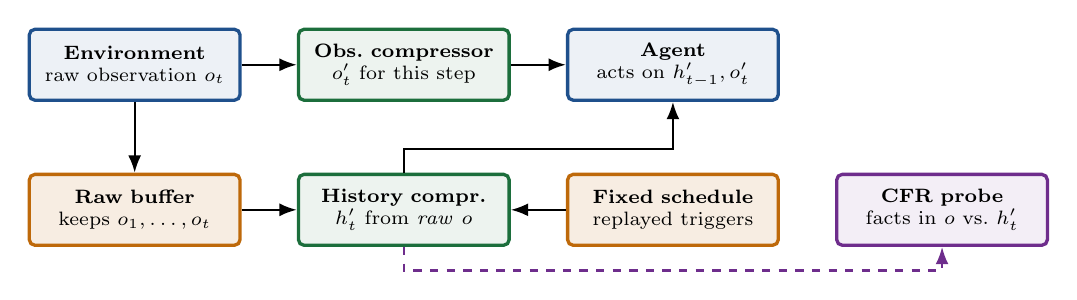
\begin{tikzpicture}[
  font=\scriptsize,
  bx/.style={draw, rounded corners=2pt, very thick, align=center,
    text width=2.5cm, minimum height=0.9cm, inner sep=2.5pt},
  arr/.style={-{Latex[length=2.2mm]}, line width=0.8pt},
  env/.style={bx, fill=envblue!8,  draw=envblue},
  cmp/.style={bx, fill=cmpgreen!8, draw=cmpgreen},
  ctl/.style={bx, fill=ctlorange!12, draw=ctlorange},
  met/.style={bx, fill=metviolet!8, draw=metviolet}
]
\node[env] (o) {\textbf{Environment}\\raw observation $o_t$};
\node[cmp, right=7mm of o]  (oc) {\textbf{Obs.\ compressor}\\$o'_t$ for this step};
\node[env, right=7mm of oc] (ag) {\textbf{Agent}\\acts on $h'_{t-1},o'_t$};
\node[ctl, below=9mm of o]  (buf){\textbf{Raw buffer}\\keeps $o_1,\dots,o_t$};
\node[cmp, right=7mm of buf](hc) {\textbf{History compr.}\\$h'_t$ from \emph{raw} $o$};
\node[ctl, right=7mm of hc] (sch){\textbf{Fixed schedule}\\replayed triggers};
\node[met, right=7mm of sch](cfr){\textbf{CFR probe}\\facts in $o$ vs.\ $h'_t$};
\draw[arr] (o)--(oc);
\draw[arr] (oc)--(ag);
\draw[arr] (o)--(buf);
\draw[arr] (buf)--(hc);
\draw[arr] (sch)--(hc);
\draw[arr] (hc.north) -- ++(0,0.3) -| (ag.south);
\draw[arr, dashed, metviolet] (hc.south) -- ++(0,-0.3) -| (cfr.south);
\end{tikzpicture}
\end{center}
\vspace{0.15cm}
\begin{columns}[T]
\begin{column}{0.49\textwidth}
\begin{block}{1. Decoupled composition order}
\footnotesize
The agent still gets the short $o'_t$, but the \textbf{raw} $o_t$ is kept in a
side buffer and $f_h$ receives $x^{\mathrm{dec}}_t$.
If $f_o$ only deletes content then $V(o'_t)\subseteq V(o_t)$, so facts dropped
by the observation stage \emph{can still reach} the history summary.
\end{block}
\end{column}
\begin{column}{0.49\textwidth}
\begin{block}{2. Controlled compression schedule}
\footnotesize
Record $\mathcal{K}^{h}=\mathcal{K}(\pi_h)$ from the history-only run and
\textbf{replay} it: $\mathcal{K}(\pi_{ho}):=\mathcal{K}^{h}$.
With the schedule fixed, $\pi_h$ and $\pi_{ho}$ differ \emph{only} in $f_o$,
so $I$ now measures composition alone.
\end{block}
\end{column}
\end{columns}
\end{frame}

% ============================== 14. CFR
\begin{frame}{3. Critical-Fact Retention: Measuring the Compressor Directly}
\begin{block}{Definition}
\footnotesize
Let $V(\cdot)$ extract state variables --- access tokens, entity IDs, file
paths, numeric values --- and let $a^{\varnothing}_{1:T}$ be the actions of the
\textbf{uncompressed reference run}. The facts at stake in trigger $t$, and the
retention rate, are
\vspace{-0.2cm}
\[
F_t=V(x_t)\cap\bigcup_{t'}V\big(a^{\varnothing}_{t'}\big),
\qquad
\mathrm{CFR}(\pi)=\frac{\sum_{t\in\mathcal{K}}\sum_{v\in F_t}
   \mathbf{1}\big[v\sqsubseteq h'_t\big]}{\sum_{t\in\mathcal{K}}|F_t|},
\]
\vspace{-0.25cm}
\footnotesize
where $v\sqsubseteq h'_t$ means an \emph{exact, verbatim} occurrence of $v$ in $h'_t$.
\end{block}

\begin{columns}[T]
\begin{column}{0.49\textwidth}
\begin{block}{Why it is cheap}
\footnotesize
\begin{itemize}
  \item $V(\cdot)$ is a set of pattern extractors for AppWorld's tokens, IDs,
        paths and numbers
  \item Computed \textbf{offline} for every compressor call
  \item \textbf{No additional agent rollouts} required
\end{itemize}
\end{block}
\end{column}
\begin{column}{0.49\textwidth}
\begin{block}{What it lets us test}
\footnotesize
\begin{itemize}
  \item Rank correlation $\rho(\mathrm{CFR},R)$ --- does fact retention
        actually predict task success?
  \item $\mathrm{CFR}$ under $x^{\mathrm{seq}}$ vs.\ $x^{\mathrm{dec}}$ ---
        does decoupling really retain more?
  \item Attribute a failure to \textbf{information loss} rather than to the
        agent
\end{itemize}
\end{block}
\end{column}
\end{columns}
\end{frame}

% ============================== 15. FUTURE WORK
\section{Future Work}

\begin{frame}{Future Work}
\begin{columns}[T]
\begin{column}{0.49\textwidth}
\begin{block}{Complete the reproduction}
\footnotesize
\begin{itemize}
  \item Finish the 38-task history-compression run
  \item Run observation and combined history\,$+$\,observation compression
  \item Add the paper thresholds ($4096/1024$) and the
        \texttt{llama3.1:8b} compressor on the same split
\end{itemize}
\end{block}
\begin{block}{Implement the proposed pipeline}
\footnotesize
\begin{itemize}
  \item Raw-observation buffer ($x^{\mathrm{dec}}$)
  \item Schedule replay $\mathcal{K}(\pi_{ho}):=\mathcal{K}^{h}$
  \item CFR extractor; then estimate $I$ under \emph{both} orders with the
        schedule held fixed
\end{itemize}
\end{block}
\end{column}
\begin{column}{0.49\textwidth}
\begin{block}{Measure latency directly}
\footnotesize
Log $\ell_M$, $\ell_{f_h}$, $\ell_{f_o}$ per call to decompose $L(\pi)$,
including \textbf{prefix re-encoding} after each history compression.
\end{block}
\begin{alertblock}{Strengthen the evidence}
\footnotesize
\begin{itemize}
  \item At least \textbf{three seeds} per setting
  \item Raise the served context window above 4096 tokens so baseline prompts
        are not truncated
  \item For SAC\,$\times$\,ACON: run \textbf{TGA alone}, plus the $5\times$ and
        $51\times$ ratios
\end{itemize}
\end{alertblock}
\end{column}
\end{columns}
\end{frame}

% ============================== 16. REFERENCES
\setbeamertemplate{bibliography item}[online]
\begin{frame}[allowframebreaks]{References}
\footnotesize
\begin{thebibliography}{9}

\bibitem{ACON} M. Kang, W.-N. Chen, D. Han, H. A. Inan, L. Wutschitz, Y. Chen,
R. Sim, and S. Rajmohan, ``ACON: Optimizing Context Compression for
Long-horizon LLM Agents,'' \emph{ICML}, PMLR 306, 2026.

\bibitem{SAC} X. Liu, R. Zhao, P. Huang, X. Liu, J. Xiao, C. Xiao, T. Xiao,
S. Gao, Z. Yu, and J. Zhu, ``Autoencoding-Free Context Compression for LLMs via
Contextual Semantic Anchors,'' \emph{ICLR}, 2026.

\bibitem{SWEPruner} Y. Wang, Y. Shi, M. Yang, R. Zhang, S. He, H. Lian,
Y. Chen, S. Ye, K. Cai, and X. Gu, ``SWE-Pruner: Self-Adaptive Context Pruning
for Coding Agents,'' arXiv:2601.16746, 2026.

\bibitem{LLMLingua} H. Jiang, Q. Wu, C.-Y. Lin, Y. Yang, and L. Qiu,
``LLMLingua: Compressing Prompts for Accelerated Inference of Large Language
Models,'' \emph{EMNLP}, pp.~13358--13376, 2023.

\bibitem{MEM1} Z. Zhou et al., ``MEM1: Learning to Synergize Memory and
Reasoning for Efficient Long-Horizon Agents,'' arXiv:2506.15841, 2025.

\bibitem{MemAgent} H. Yu et al., ``MemAgent: Reshaping Long-Context LLM with
Multi-Conv RL-based Memory Agent,'' \emph{ICLR}, 2026.

\bibitem{AppWorld} H. Trivedi et al., ``AppWorld: A Controllable World of Apps
and People for Benchmarking Interactive Coding Agents,'' \emph{ACL},
pp.~16022--16076, 2024.

\end{thebibliography}
\end{frame}

% ============================== 17. THANK YOU
{
\setbeamertemplate{footline}{}
\begin{frame}[plain]
\vspace{1.0cm}
\begin{center}
  \includegraphics[height=1.5cm]{"png college logo".png}

  \vspace{0.7cm}
  {\Huge\bfseries\color{envblue} Thank You}

  \vspace{0.5cm}
  \rule{0.45\textwidth}{0.8pt}

  \vspace{0.5cm}
  {\Large Questions?}

  \vspace{1.0cm}
  \footnotesize
  \begin{tabular}{r@{\hspace{0.8em}}l}
    \textbf{123CS0006} & Ayush Rahate\\
    \textbf{123CS0054} & Rohit Chauhan
  \end{tabular}

  \vspace{0.4cm}
  \footnotesize Supervisor: Dr.~N.~Srinivas Naik
\end{center}
\end{frame}
}

\end{document}
